\documentclass{article}
\usepackage{amsmath, amssymb, amsthm}
\usepackage{tikz}
\usetikzlibrary{graphs,graphs.standard}

\begin{document}

\title{Matrices de Adyacencia e Incidencia}
\author{David Rivera Morales}
\maketitle

\section*{Gráfica \( G_1 \)}

\begin{center}
	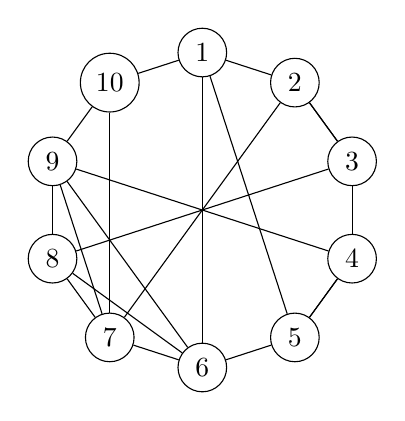
\begin{tikzpicture}
		\graph [nodes={draw, circle}, clockwise] {
		subgraph C_n [n=10, name=A, radius=2cm];
		A 1 -- A 5; A 1 -- A 6;
		A 2 -- A 3; A 2 -- A 7;
		A 3 -- A 4; A 3 -- A 8;
		A 4 -- A 5; A 4 -- A 9;
		A 6 -- A 8; A 6 -- A 9;
		A 7 -- A 9; A 7 -- A 10;
		};
	\end{tikzpicture}
\end{center}

Justificación:
\begin{itemize}
	\item \( G_1 \) tiene 10 vértices.
	\item Los grados de los vértices de \( G_1 \) son: 3, 2, 2, 3, 1, 3, 3, 1, 0, 0.
\end{itemize}

\begin{array}{c|l}
	\text{Vertex} & \text{Adjacent Vertices} \\
	\hline
	v1            & v2, v5, v6               \\
	v2            & v3, v7                   \\
	v3            & v4, v8                   \\
	v4            & v5, v9                   \\
	v5            & v10                      \\
	v6            & v8, v9                   \\
	v7            & v9, v10                  \\
	v8            & v10                      \\
	v9            &                          \\
	v10           &                          \\
\end{array}


\textbf{Matriz de Adyacencia \( G_1 \)}:
\[
A_1 =
\begin{array}{c|cccccccccc}
    & v1 & v2 & v3 & v4 & v5 & v6 & v7 & v8 & v9 & v10 \\
\hline
v1 & 0 & 1 & 0 & 0 & 1 & 1 & 0 & 0 & 0 & 0 \\
v2 & 0 & 0 & 1 & 0 & 0 & 0 & 1 & 0 & 0 & 0 \\
v3 & 0 & 0 & 0 & 1 & 0 & 0 & 0 & 1 & 0 & 0 \\
v4 & 0 & 0 & 0 & 0 & 1 & 0 & 0 & 0 & 1 & 0 \\
v5 & 0 & 0 & 0 & 0 & 0 & 0 & 0 & 0 & 0 & 1 \\
v6 & 0 & 0 & 0 & 0 & 0 & 0 & 0 & 1 & 1 & 0 \\
v7 & 0 & 0 & 0 & 0 & 0 & 0 & 0 & 0 & 1 & 1 \\
v8 & 0 & 0 & 0 & 0 & 0 & 0 & 0 & 0 & 0 & 1 \\
v9 & 0 & 0 & 0 & 0 & 0 & 0 & 0 & 0 & 0 & 0 \\
v10& 0 & 0 & 0 & 0 & 0 & 0 & 0 & 0 & 0 & 0 \\
\end{array}
\]


\textbf{Matriz de Incidencia \( G_1 \)}:

\setcounter{MaxMatrixCols}{20}
\[
M_1 =
\begin{array}{c|ccccccccccccccc}
    & e1 & e2 & e3 & e4 & e5 & e6 & e7 & e8 & e9 & e10 & e11 & e12 & e13 & e14 & e15 \\
\hline
v1 & 1  & 1  & 1  & 0  & 0  & 0  & 0  & 0  & 0  & 0  & 0  & 0  & 0  & 0  & 0   \\
v2 & -1 & 0  & 0  & 1  & 1  & 0  & 0  & 0  & 0  & 0  & 0  & 0  & 0  & 0  & 0   \\
v3 & 0  & 0  & 0  & -1 & 0  & 1  & 1  & 0  & 0  & 0  & 0  & 0  & 0  & 0  & 0   \\
v4 & 0  & 0  & 0  & 0  & 0  & -1 & 0  & 1  & 1  & 0  & 0  & 0  & 0  & 0  & 0   \\
v5 & 0  & -1 & 0  & 0  & 0  & 0  & 0  & -1 & 0  & 1  & 0  & 0  & 0  & 0  & 0   \\
v6 & 0  & 0  & -1 & 0  & 0  & 0  & 0  & 0  & 0  & 0  & 1  & 1  & 0  & 0  & 0   \\
v7 & 0  & 0  & 0  & 0  & -1 & 0  & 0  & 0  & 0  & 0  & 0  & 0  & 1  & 1  & 0   \\
v8 & 0  & 0  & 0  & 0  & 0  & 0  & -1 & 0  & 0  & 0  & -1 & 0  & 0  & 0  & 1   \\
v9 & 0  & 0  & 0  & 0  & 0  & 0  & 0  & 0  & -1 & 0  & 0  & -1 & -1 & 0  & 0   \\
v10& 0  & 0  & 0  & 0  & 0  & 0  & 0  & 0  & 0  & -1 & 0  & 0  & 0  & -1 & -1  \\
\end{array}
\]

\section*{Gráfica \( G_2 \)}

\begin{center}
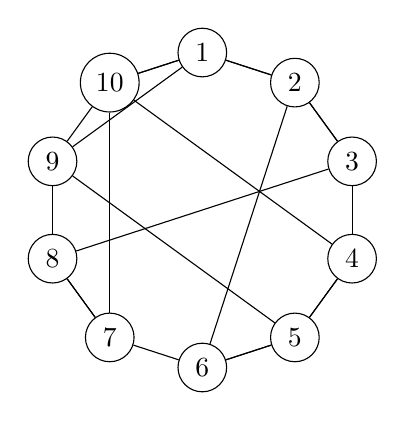
\begin{tikzpicture}
    \graph [nodes={draw, circle}, clockwise] {
        subgraph C_n [n=10, name=B, radius=2cm];
        B 1 -- B 2; B 1 -- B 9; B 1 -- B 10;
        B 2 -- B 3; B 2 -- B 6;
        B 3 -- B 4; B 3 -- B 8;
        B 4 -- B 5; B 4 -- B 10;
        B 5 -- B 6; B 5 -- B 9;
        B 7 -- B 8; B 7 -- B 10;
    };
\end{tikzpicture}
\end{center}

Justificación:
\begin{itemize}
    \item \( G_2 \) tiene 10 vértices.
    \item Los grados de los vértices de \( G_2 \) son: 3, 2, 2, 3, 2, 1, 3, 1, 0, 0.
    \item \( G_1 \) no es isomorfa a \( G_2 \) ya que, aunque tienen el mismo número de vértices y aristas, sus conjuntos de grados de vértices son diferentes.
\end{itemize}


\begin{array}{c|l}
	\text{Vertex} & \text{Adjacent Vertices} \\
	\hline
	v1            & v2, v9, v10              \\
	v2            & v3, v6                   \\
	v3            & v4, v8                   \\
	v4            & v5, v10                  \\
	v5            & v6,v9                    \\
	v6            & v7                       \\
	v7            & v8, v10                  \\
	v8            & v9                       \\
	v9            &                          \\
	v10           &                          \\
\end{array}

\textbf{Matriz de Adyacencia \( G_2 \)}:
\[
A_2 =
\begin{array}{c|cccccccccc}
    & v1 & v2 & v3 & v4 & v5 & v6 & v7 & v8 & v9 & v10 \\
\hline
v1 & 0 & 1 & 0 & 0 & 0 & 0 & 0 & 0 & 1 & 1 \\
v2 & 0 & 0 & 1 & 0 & 0 & 1 & 0 & 0 & 0 & 0 \\
v3 & 0 & 0 & 0 & 1 & 0 & 0 & 0 & 1 & 0 & 0 \\
v4 & 0 & 0 & 0 & 0 & 1 & 0 & 0 & 0 & 0 & 1 \\
v5 & 0 & 0 & 0 & 0 & 0 & 1 & 0 & 0 & 1 & 0 \\
v6 & 0 & 0 & 0 & 0 & 0 & 0 & 1 & 0 & 0 & 0 \\
v7 & 0 & 0 & 0 & 0 & 0 & 0 & 0 & 1 & 0 & 1 \\
v8 & 0 & 0 & 0 & 0 & 0 & 0 & 0 & 0 & 1 & 0 \\
v9 & 0 & 0 & 0 & 0 & 0 & 0 & 0 & 0 & 0 & 0 \\
v10& 0 & 0 & 0 & 0 & 0 & 0 & 0 & 0 & 0 & 0 \\
\end{array}
\]

\textbf{Matriz de Incidencia \( G_2 \)}:

\setcounter{MaxMatrixCols}{20}
\[
M_2 =
\begin{array}{c|ccccccccccccccc}
    & e1 & e2 & e3 & e4 & e5 & e6 & e7 & e8 & e9 & e10 & e11 & e12 & e13 & e14 & e15 \\
\hline
v1 & 1  & 1  & 1  & 0  & 0  & 0  & 0  & 0  & 0  & 0  & 0  & 0  & 0  & 0  & 0   \\
v2 & -1 & 0  & 0  & 1  & 1  & 0  & 0  & 0  & 0  & 0  & 0  & 0  & 0  & 0  & 0   \\
v3 & 0  & 0  & 0  & -1 & 0  & 1  & 1  & 0  & 0  & 0  & 0  & 0  & 0  & 0  & 0   \\
v4 & 0  & 0  & 0  & 0  & 0  & -1 & 0  & 1  & 1  & 0  & 0  & 0  & 0  & 0  & 0   \\
v5 & 0  & 0  & 0  & 0  & 0  & 0  & 0  & -1 & 0  & 1  & 1  & 0  & 0  & 0  & 0   \\
v6 & 0  & 0  & 0  & 0  & -1 & 0  & 0  & 0  & 0  & -1 & 0  & 1  & 0  & 0  & 0   \\
v7 & 0  & 0  & 0  & 0  & 0  & 0  & 0  & 0  & 0  & 0  & 0  & -1 & 1  & 1  & 0   \\
v8 & 0  & 0  & 0  & 0  & 0  & 0  & -1 & 0  & 0  & 0  & 0  & 0  & -1 & 0  & 1   \\
v9 & 0  & -1 & 0  & 0  & 0  & 0  & 0  & 0  & 0  & 0  & -1 & 0  & 0  & 0  & -1  \\
v10& 0  & 0  & -1 & 0  & 0  & 0  & 0  & 0  & -1 & 0  & 0  & 0  & 0  & -1 & 0   \\
\end{array}
\]

\section*{Gráfica \( G_3 \)}

\begin{center}
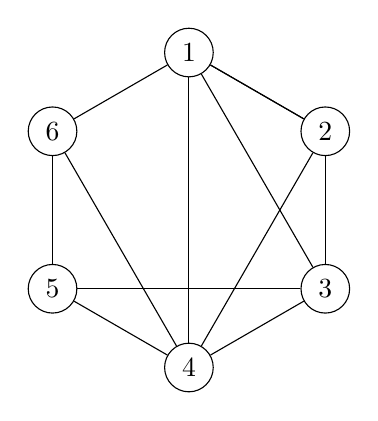
\begin{tikzpicture}
    \graph [nodes={draw, circle}, clockwise] {
        subgraph C_n [n=6, name=C, radius=2cm];
        C 1 -- C 2; C 1 -- C 3; C 1 -- C 4;
        C 2 -- C 4;
        C 3 -- C 5;
        C 4 -- C 6;
        C 5 -- C 6;
    };
\end{tikzpicture}
\end{center}

Justificación:
\begin{itemize}
    \item \( G_3 \) tiene 6 vértices.
    \item Los grados de los vértices de \( G_3 \) son: 3, 1, 2, 2, 1, 0.
\end{itemize}

\begin{array}{c|l}
	\text{Vertex} & \text{Adjacent Vertices} \\
	\hline
	x1            & x2, x3, x4               \\
	x2            & x4                       \\
	x3            & x5                       \\
	x4            & x5, x6                   \\
	x5            & x6                       \\
	x6            &                          \\
\end{array}

\textbf{Matriz de Adyacencia \( G_3 \)}:
\[
A_3 =
\begin{array}{c|cccccc}
    & x1 & x2 & x3 & x4 & x5 & x6 \\
\hline
x1 & 0 & 1 & 1 & 1 & 0 & 0 \\
x2 & 0 & 0 & 0 & 1 & 0 & 0 \\
x3 & 0 & 0 & 0 & 0 & 1 & 0 \\
x4 & 0 & 0 & 0 & 0 & 1 & 1 \\
x5 & 0 & 0 & 0 & 0 & 0 & 1 \\
x6 & 0 & 0 & 0 & 0 & 0 & 0 \\
\end{array}
\]


\textbf{Matriz de Incidencia \( G_3 \)}:
\[
M_3 =
\begin{array}{c|cccccccc}
    & e1 & e2 & e3 & e4 & e5 & e6 & e7 & e8 \\
\hline
x1 & 1  & 1  & 1  & 0  & 0  & 0  & 0  & 0  \\
x2 & -1 & 0  & 0  & 1  & 0  & 0  & 0  & 0  \\
x3 & 0  & 0  & 0  & -1 & 1  & 0  & 0  & 0  \\
x4 & 0  & 0  & 0  & 0  & -1 & 1  & 1  & 0  \\
x5 & 0  & 0  & 0  & 0  & 0  & 0  & 0  & 1  \\
x6 & 0  & -1 & -1 & 0  & 0  & -1 & -1 & -1 \\
\end{array}
\]


\section*{Gráfica \( G_4 \)}

\begin{center}
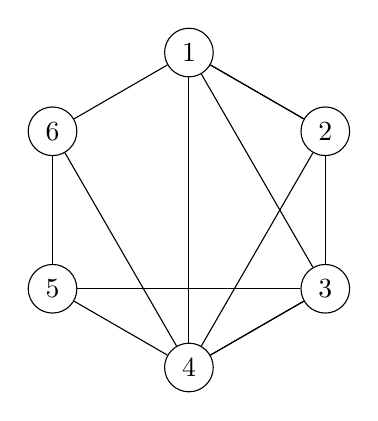
\begin{tikzpicture}
    \graph [nodes={draw, circle}, clockwise] {
        subgraph C_n [n=6, name=D, radius=2cm];
        D 1 -- D 2; D 1 -- D 3; D 1 -- D 4;
        D 2 -- D 4;
        D 3 -- D 4; D 3 -- D 5;
        D 4 -- D 6;
        D 5 -- D 6;
    };
\end{tikzpicture}
\end{center}

Justificación:
\begin{itemize}
    \item \( G_4 \) tiene 6 vértices.
    \item Los grados de los vértices de \( G_4 \) son: 3, 1, 2, 2, 1, 0.
    \item \( G_3 \) es potencialmente isomorfa a \( G_4 \) ya que tienen el mismo número de vértices, el mismo número de aristas y el mismo conjunto de grados de vértices. 
\end{itemize}

\begin{array}{c|l}
	\text{Vertex} & \text{Adjacent Vertices} \\
	\hline
	w1            & w2, w3, w4               \\
	w2            & w4                       \\
	w3            & w4,w5                    \\
	w4            & w6                       \\
	w5            & w6                       \\
	w6            &                          \\
\end{array}


\textbf{Matriz de Adyacencia \( G_4 \)}:
\[
A_4 =
\begin{array}{c|cccccc}
    & w1 & w2 & w3 & w4 & w5 & w6 \\
\hline
w1 & 0 & 1 & 1 & 1 & 0 & 0 \\
w2 & 0 & 0 & 0 & 1 & 0 & 0 \\
w3 & 0 & 0 & 0 & 1 & 1 & 0 \\
w4 & 0 & 0 & 0 & 0 & 0 & 1 \\
w5 & 0 & 0 & 0 & 0 & 0 & 1 \\
w6 & 0 & 0 & 0 & 0 & 0 & 0 \\
\end{array}
\]


\textbf{Matriz de Incidencia \( G_4 \)}:
\[
M_4 =
\begin{array}{c|cccccccc}
    & e1 & e2 & e3 & e4 & e5 & e6 & e7 & e8 \\
\hline
w1 & 1  & 1  & 1  & 0  & 0  & 0  & 0  & 0  \\
w2 & -1 & 0  & 0  & 1  & 0  & 0  & 0  & 0  \\
w3 & 0  & 0  & 0  & 0  & 1  & 1  & 0  & 0  \\
w4 & 0  & 0  & 0  & -1 & 0  & 0  & 1  & 0  \\
w5 & 0  & 0  & 0  & 0  & -1 & 0  & 0  & 1  \\
w6 & 0  & 0  & 0  & 0  & 0  & -1 & -1 & -1 \\
\end{array}
\]



\end{document}
